% -*- TeX:de -*-
\NeedsTeXFormat{LaTeX2e}
\documentclass[12pt,a4paper,titlepage]{article}

%\usepackage[german]{babel} % german text
\usepackage[DIV12]{typearea} % size of printable area
\usepackage[T1]{fontenc} % font encoding
\usepackage[utf8]{inputenc} % probably on Linux

\usepackage{graphicx} % to include images
\graphicspath{ {img/} } % set default image directory
\usepackage{subfigure} % for creating subfigures
\usepackage{amsmath} % a bunch of symbols
\usepackage{amssymb} % even more symbols
\usepackage{booktabs} % pretty tables
\usepackage{csquotes}

% a floating environment for circuits
\usepackage{float}
\usepackage{caption}

\newfloat{circuit}{tbph}{circuits}
\floatname{circuit}{Schaltplan}

% a floating environment for diagrams
\newfloat{diagram}{tbph}{diagrams}
\floatname{diagram}{Diagramm}

\renewcommand{\familydefault}{\sfdefault} % activate to use sans-serif font as default

\sloppy % friendly typesetting

\usepackage{eurosym}
\usepackage{makeidx}
\usepackage{amsfonts}
\usepackage{mparhack}
\usepackage{array}
\usepackage{tabularx}
\usepackage{minitoc}
\usepackage[colorlinks=true]{hyperref}
\usepackage{epstopdf}
\usepackage{setspace}
\usepackage{csquotes}
\usepackage{circuitikz}

% hyperref settings
\hypersetup{
    colorlinks=false,       % false: boxed links; true: colored links
    linkcolor=black,          % color of internal links (change box color with linkbordercolor)
    citecolor=black,        % color of links to bibliography
    filecolor=black,      % color of file links
    urlcolor=black           % color of external links
}

\begin{document}

\begin{titlepage}

\begin{figure*}[h!]
  
\includegraphics[width=8cm]{TULogo_CMYK}
\end{figure*}

\begin{center}
\vspace*{1.3cm}
{\Huge Elektrotechnische Grundlagen der Informatik\\(LU 182.692)\\}
\vspace{1.7cm}
{\LARGE Protokoll der 4. Laborübung: \enquote{Spektren}\\}
\vspace{1.7cm}

% fill in group number and date of lab here
% CHANGE ME!
{\Large Gruppennr.: 22 \hspace{1cm} Datum der Laborübung: 21.0.6.2017}

% fill in IDs and names here
% CHANGE ME!
\begin{table}[h!]
\centering
\begin{tabular}{|p{3.5cm}|p{3.5cm}|p{6.5cm}|}
\hline \textbf{Matr. Nr.} & \textbf{Kennzahl} & \textbf{Name} \\
\hline
1614835 & 033 535 & Jan Nausner \\
\hline
1633068 & 033 535 & David Pernerstorfer \\
\hline
\end{tabular}
\end{table}

\end{center}
\vspace{1.0cm}

\begin{table}[h!]
\begin{tabular}{|l|l|}
\hline \textbf{Kontrolle} & \checkmark \\
\hline Sinus-Signal im Frequenzbereich & \\
\hline Rechteck-Signal im Frequenzbereich & \\
\hline Amplitudenmodulation & \\
\hline Brückengleichrichter & \\
\hline
\end{tabular}
\end{table}

\end{titlepage}

\setcounter{page}{2}

\newpage
\setcounter{tocdepth}{1}
\tableofcontents

\newpage

\section*{Materialien}
\begin{itemize}
	\item Oszilloskop: Agilent InfiniiVision MSO-X 3054A
	\item Frequenzgenerator: Agilent 33220A
\end{itemize}

\section{Messung eines Sinussignals im Spektralbereich mittels FFT}

%\subsection*{Notizen}
% Eingangssignal: Sinus $100kHz$, $1V_{pp}$, $V_{offset}=0V$ \\
% Aufzeichnung Signal im Zeitbereich scope\_18/19, kein Aliasing \\
% \\
% Aufzeichung im FQ bereich: Einstellungen: Taste Math;
%
% logarithmisch (spanne 200kHz, center 100kHz):
% Hanning-Fenster: scope_20/21
% Rechteck-Fenster: scope_22/23
% BLackmann-Harris: scope_24/25
% Rechteck: scope_30/31 spanne 10kHz, center 100kHz
% Rechteck: scope_34 spanne 10kHz, center 100kHz Messung
% Blackman-Harris: scope_35 spanne 10kHz, center 100kHz Messung
% Blackman-Harris: scope_36 spanne 10kHz, center 100kHz Messung, Amplitude
%
% linear:
% Rechteck: scope_26/27 spanne 1kHz, center 100kHz
% Rechteck: scope_28/29 spanne 10kHz, center 100kHz
% Blackman-Harris: scope_32/ spanne 10kHz, center 100kHz Messung
% Rechteck: scope_33 spanne 10kHz, center 100kHz Messung
% Blackman-Harris: scope_37 spanne 10kHz, center 100kHz Messung, Amplitude
%
% Messung: Amplitude: -9.2dB = 20*log_10(Veff/1V) = 20*log_10(0.5*1/sqrt(2))

\subsection*{Aufgabenstellung}
Ein einfaches Sinussignal soll im Zeit- und Frequenzbereich grafisch dargestellt werden.

\subsection*{Durchf\"uhrung}
Das Oszilloskop wurde direkt mit dem Funktionsgeneraor verbunden und mit diesem wurde daraufhin ein Sinussignal mit $1 V_{pp}$ und $100kHz$ Frequenz erzeugt. Das Bild im Zeitbereich wurde aufgenommen. danach wurde das Signal mittels FFT-Funktion in den Frequenzbereich transformiert und ebenfalls wieder aufgenommen.

\subsection*{Ergebnisse \& Diskussion}
\begin{figure}[H]
  \centering
  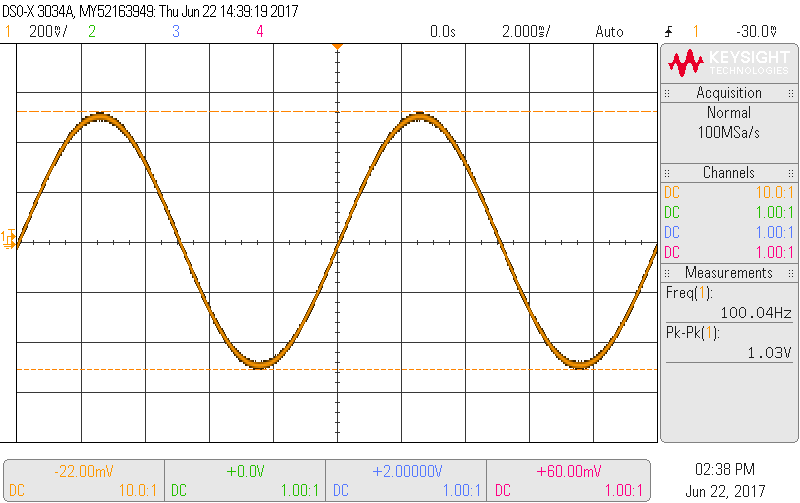
\includegraphics[width=150mm]{scope_18.png}
  \caption{Sinussignal mit $1V_{pp}$ und $100kHz$ im Zeitbereich}
\end{figure}

\begin{figure}[H]
  \centering
  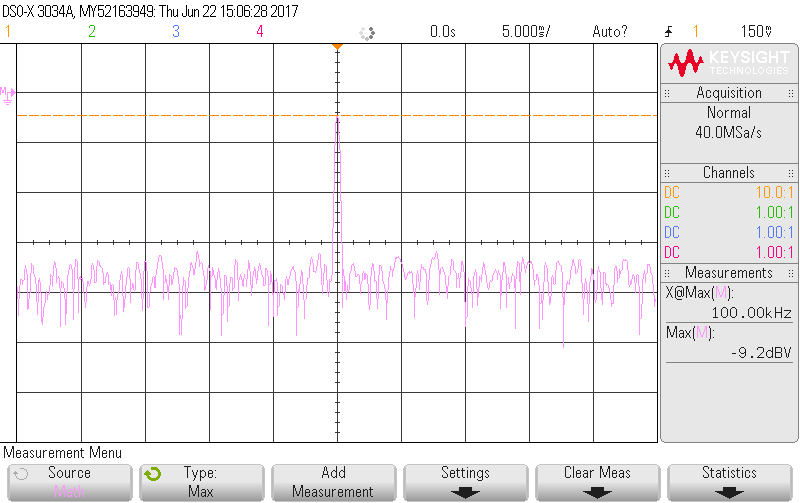
\includegraphics[width=150mm]{scope_36.png}
  \caption{Sinussignal mit $1V_{pp}$ und $100kHz$ im Frequenzbereich (logarithmische Darstellung)}
\end{figure}

\noindent Bei der Darstellung im Frequenzbereich kann man sehr gut die charakteristische (und einzige) Spektrallinie des Sinussignals bei der Frequenz $100kHz$ (Signalfrequenz) erkennen. Unter Anderem durch die Abtastung und die diskrete Signalanalyse kommt es zu Rauschen, welches durch die logarithmische Darstellung verstärkt sichtbar wird. Die Spektrallinie des Sinus hat hier eine Amplitude von $-9,2dB$, was ungefähr der logarithmischen Darstellung des Effektivwerts des Signals entspricht ($20 \cdot log_{10} (\frac{V_{rms}}{1V}) = 20 \cdot log_{10} \left(\frac{\frac{0,5V}{\sqrt{2}}}{1V}\right) \approx -9dB$). Der Fehler von ca. $2\%$ stammt auch hier aus der Abtastung und der digitalen Signalanalyse.\\

\noindent Bei der Frequenzdarstellung mittels FFT ist es wichtig, eine geeignete Fensterfunktion zu wählen. Diese bestimmt, welche Eigenschaft des Signals sehr genau gemessen wird und wo es unter Umständen zu Ungenauigkeiten kommen kann. Hier muss man zwischen minimalem Leck-Effekt, genauer Amplitudenmessung und scharfer Frequenzmessung wählen. Hier wurde das Blackman-Harris-Fenster gewählt. Um ein Aussagekräftiges Spektrum zu erhalten, ist es auch notwendig, eine geeignete Frequenzbandbreite darzustellen (hier $10kHz$) und wichtige Frequenzanteile zu zentrieren.

\begin{figure}[H]
  \centering
  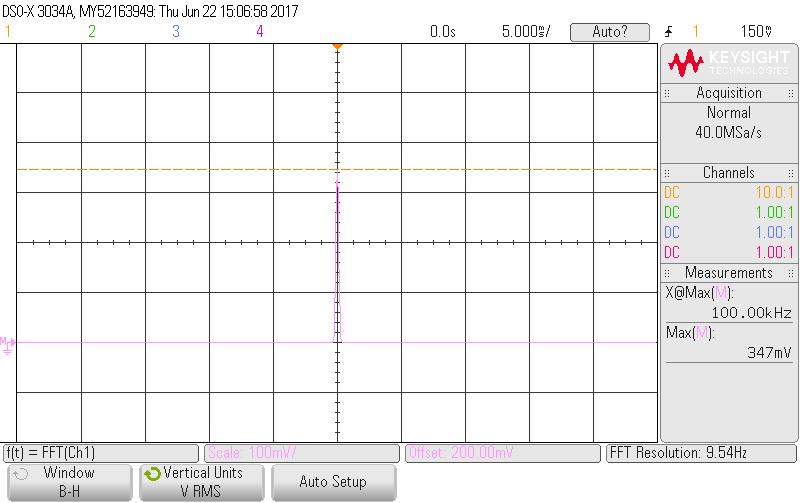
\includegraphics[width=150mm]{scope_37.png}
  \caption{Sinussignal mit $1V_{pp}$ und $100kHz$ im Frequenzbereich (lineare Darstellung)}
\end{figure}

\noindent Auch bei der linearen Darstellung der Amplitude ist die Spektrallinie bei $100kHz$ mit $347mV_{rms}$ gut zu sehen. Hierbei fällt auf, dass das Rauschen nicht mehr sichtbar ist. Jedoch kann es hierbei sein, dass kleine Frequenzanteile ebenfalls nicht mehr sichtbar sind. Daher wird in der Praxis meist die logarithmische Darstellung benutzt.

\section{Messung eines Rechtecksignals}

\subsection*{Notizen}
% FQ Generator Einstellungen: Square $50\%$ duty circle $10kHz$, $1V_{pp}$ \\
% Rechtecksignal im Zeitbereich: scope_40 \\
% Hanning; Vrms; spanne 100kHz, center 50kHz; Vrm $450mV$; scope_39 \\
% Hauptkomponente gemessen mit Cursor: $10kHz$, $450mV$ \\
% 1. Nebenkomponente: $30kHz$, $147mV$
% 2. Nebenkomponente: $50kHz$, $94mV$
% 3. Nebenkomponente: $70kHz$, $65mV$

\subsection*{Schaltplan}
% \begin{figure}[H]
%   \centering
%   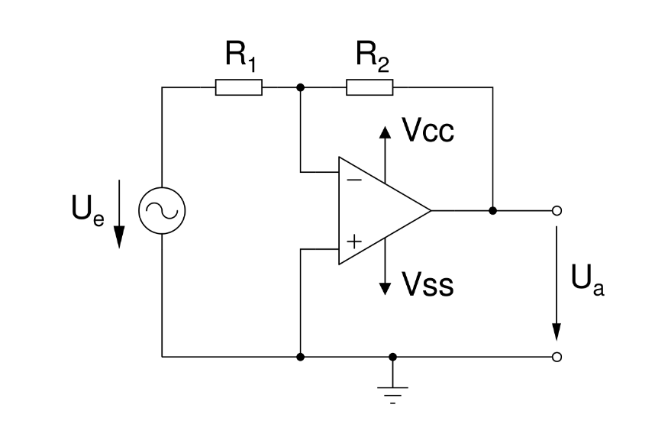
\includegraphics[width=100mm]{i_opv_schaltung.png}
%   \caption{Invertierender OPV}
% \end{figure}

\subsection*{Durchf\"uhrung}

\subsection*{Ergebnisse \& Diskussion}

\section{Amplitudenmodulation}

\subsection*{Notizen}
% Einstellungen FQ Generator: \\
%
% Tr\"agerfq: Sinus $100kHz$, $1V_{pp}$ \\
% Nutzsignal: Sinus $1kHz$, Gleichanteil $0V$ \\
% Zeitbereich scope_41 \\
% Zeitbereich scope_42 \\
% Hanning-Fenster am Oszi
%
% Frequenzbereich: scope_43, linear
% scope_47 logarithmisch
% scope_48 logarithmisch (rectangle)
% Hauptkomponente: 100kHz, Amplitude 166,92mV
% Linke Nebenkomponente: 99kHz, 86mV
% Rechte Nebenkomponente: 101kHz, 86mV
%
% Einstellungen FQ Generator: \\
% Tr\"agerfq: Sinus $100kHz$, $1V_{pp}$ \\
% Nutzsignal: Rechteck $1kHz$, Gleichanteil $0V$ \\
% Zeitbereich scope_44 \\
%
% Frequenzbereich: scope_45, linear
% scope_46 logarithmisch
% Hauptkomponente: 100kHz, Amplitude 175mV
% 1. Linke Nebenkomponente: 99kHz, 111mV
% 2. Linke Nebenkomponente: 97kHz, 37mV
% 3. Linke Nebenkomponente: 95kHz, 23mV
% 4. Linke Nebenkomponente: 93kHz, 16mV
% 1. R Nebenkomponente: 101kHz, 111mV
% 2. R Nebenkomponente: 103kHz, 37mV
% 3. R Nebenkomponente: 105kHz, 23mV
% 4. R Nebenkomponente: 107kHz, 16mV

\subsection*{Aufgabenstellung}


\subsection*{Schaltplan}
% \begin{figure}[H]
%   \centering
%   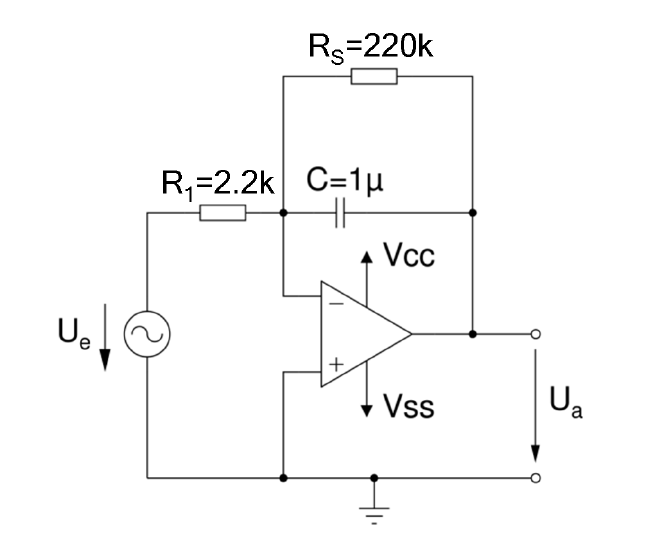
\includegraphics[width=80mm]{integrierer_opv_schaltung.png}
%   \caption{Integrierer}
%   \label{figure31}
% \end{figure}

\subsection*{Durchf\"uhrung}


\subsection*{Ergebnisse \& Diskussion}

\section{Brückengleichrichter}

\subsection*{Notizen}
% Dioden N4148, Widerstand $1MOhm$ \\
%
% Frequenzgenerator $2V_{pp}$, $1kHz$
% Zeitbereich: ($U_a$) $scope_52$, $scope_53$ \\
% Messung $U_a$ $520mV_PP$ $DC_{rms}=338mV$ $Fq=2kHz$ \\
% \\
% Frequenzgenerator $10V_{pp}$, $1kHz$
% Zeitbereich: ($U_a$) $scope_54$ \\
% Messung $U_a$ $4,22V_PP$ $DC_{rms}=2,91V$ $Fq=2kHz$ \\
% \\
%
%
% Frequenzbereich:
% Spektrum scope_57 (rectangle), logarithmisch \\
% Hauptkomponente: $2kHz$, $3,13dB$ \\
% 1. Nebenkomponente: $4kHz$, $-11,27dB$ \\
% 2. Nebenkomponente: $6kHz$, $-21,9dB$ \\
% 3. Nebenkomponente: $8kHz$, $-27,86dB$ \\
% 4. Nebenkomponente: $10kHz$, $-37,25dB$


\subsection*{Aufgabenstellung}
Das Ausgangssignal eines Brückengleichrichters soll sowohl im Zeit-, als auch im Frequentbereich gemessen und mit der dazugehörigen Fourierreihe verglichen werden.

\subsection*{Schaltplan}
\begin{figure}[H]
  \centering
  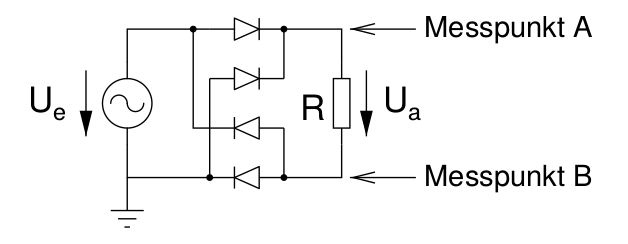
\includegraphics[width=100mm]{bg_schaltung.png}
  \caption{Brückengleichrichter}
  \label{figure41}
\end{figure}

\subsection*{Durchf\"uhrung}
Die Schlatung wurde gemäß Schaltplan mit 4 1N4148 Dioden und einem $1M\Omega$ Widerstand aufgebaut. Da der Ausgang des Brückengleichrichters nicht auf Masse liegt, musste die Spannung an diesem mit zwei Oszilloskopkanälen (A und B) gemessen werden. Die Differenz $A - B$ entspricht hier dem Ausgangssignal. Im Zeitbereich wurde ein gleichgerichteter Sinus mit $1kHz$ Frequenz und $2$ bzw. $10V_{pp}$ gemessen. Das Signal mit $10V_{pp}$ wurde mittels FFT (Hannuing-Fenster) auch im Spektralbereich dargestellt. Um Vergleiche zu ermöglichen wurde die Fourrierreihe zu $|sin(\omega t)|$ berechnet.

\subsection*{Ergebnisse \& Diskussion}

\begin{figure}[H]
  \centering
  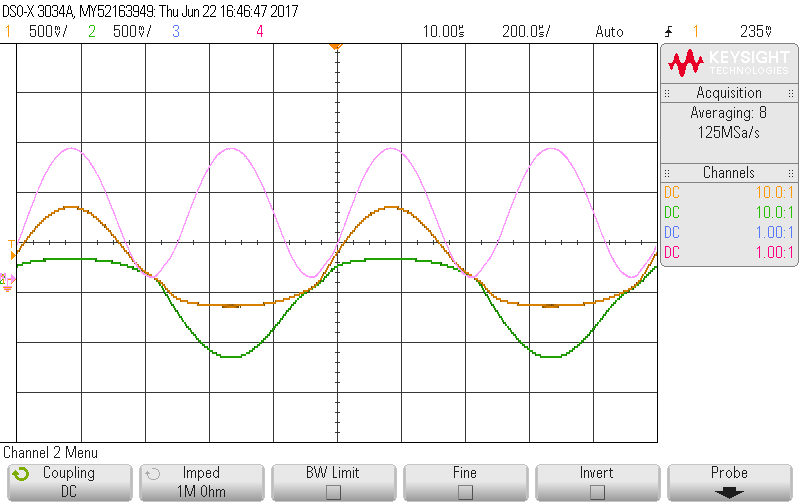
\includegraphics[width=150mm]{scope_52.png}
  \caption{Gleichgerichteter Sinus (violett) (Eingangssignal $10kHz$, $2V_{pp}$, gelb $\hdots$ Messpunkt A, grün $\hdots$ Messpunkt B)}
\end{figure}

\noindent Hier lässt sich gut erkennen, dass durch die Brückengleichrichterschaltung die negativen Halbwellen des Sinussignals in den positiven Bereich "geklappt" werden. Dadurch wird die Frequenz doppelt so hoch ($2kHz$) als die der Eingangsspannung. Die Spitzenspannung beträgt hier $520mV$ und der Effektivwert $338mV$. Der Unterschied zur Spitzenspannung des theoretischen Ausgangssignals ($1V$) lässt sich dadurch erklären, dass das Signal bei der Gleichrichtung immer 2 Dioden durchfließen und somit deren Schwellspannung überwinden muss.

\begin{figure}[H]
  \centering
  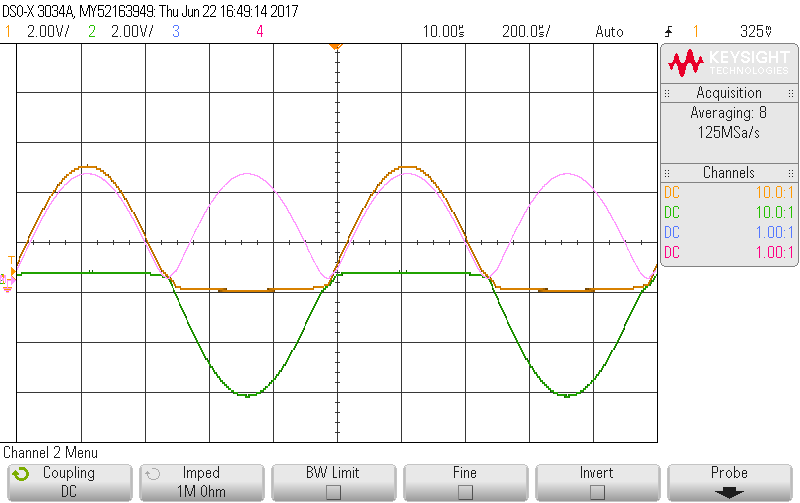
\includegraphics[width=150mm]{scope_54.png}
  \caption{Gleichgerichteter Sinus (violett) (Eingangssignal $10kHz$, $10V_{pp}$, gelb $\hdots$ Messpunkt A, grün $\hdots$ Messpunkt B)}
\end{figure}

\noindent Bei einem Sinussignal mit $10V_{pp}$ wurden $4,22V$ Spitzenspannung und $2,91V_{RMS}$ gemessen.

\begin{figure}[H]
  \centering
  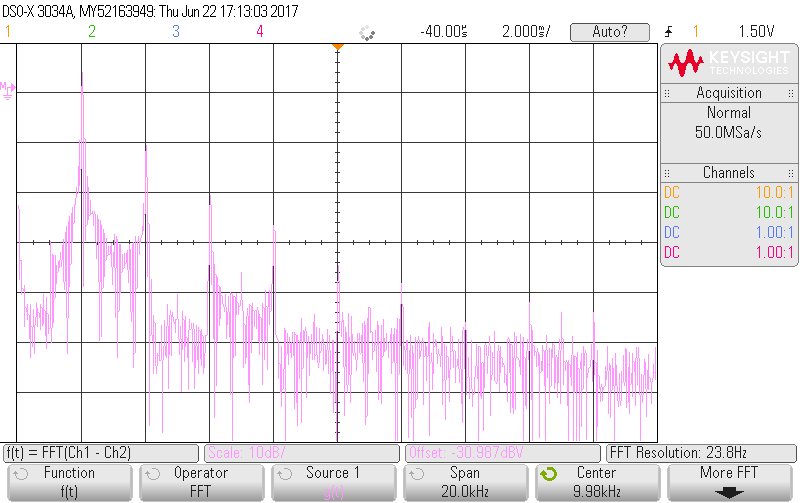
\includegraphics[width=150mm]{scope_57.png}
  \caption{Spektrum des gleichgerichteten Sinus (logarithmische Darstellung)}
\end{figure}

\noindent Die Spketrallinien liegen hier bei ganzzahligen Vielfachen der Frundfrequenz des gleichgerichteten Sinus ($2kHz$).

% Hauptkomponente: $2kHz$, $3,13dB$ \\
% 1. Nebenkomponente: $4kHz$, $-11,27dB$ \\
% 2. Nebenkomponente: $6kHz$, $-21,9dB$ \\
% 3. Nebenkomponente: $8kHz$, $-27,86dB$ \\
% 4. Nebenkomponente: $10kHz$, $-37,25dB$

\begin{table}[H]
  \centering
  \begin{tabular}{c|c|c}
    $f [kHz]$ & Amplitude $[dB]$ & Amplitude $[V_{rms}]$ \\
    \hline
    $2$ & $3,13$ & $1,43$ \\
    \hline
    $4$ & $-11,27$ & $0,27$ \\
    \hline
    $6$ & $-21,9$ & $0,08$ \\
    \hline
    $8$ & $-27,86$ & $0,04$ \\
    \hline
    $10$ & $-37,25$ & $0,01$ \\
  \end{tabular}
  \caption{Messung der 5 größten Spektralkomponenten}
\end{table}

\noindent Berechnung der Fourierreihe des gleichgerichteten Sinus:\\
\begin{align*}
    a_n &= \frac{2}{\pi}\int_{0}^{\pi}sin(t)\cdot cos(nt) dt\\
    &= \frac{1}{\pi}\int_{0}^{\pi}\left[sin(t - nt) + sin(t + nt)\right] dt\\
    &= \frac{1}{\pi}\left[\frac{1}{n-1}cos(t(1-n)) - \frac{1}{1+n}cos(t(1+n))\right]\biggr\rvert_{0}^{\pi}\\
    &= \frac{1}{\pi}\left[\frac{1}{n-1}cos(\pi-n\pi) - \frac{1}{1+n}cos(n\pi + \pi) - \frac{1}{n-1} + \frac{1}{1+n}\right]\\
    &= \frac{2cos(n\pi + \pi) - 2}{\pi(n+1)(n-1)} = \left\{
	    \begin{array}{ll}
		     0  & n \; ungerade \\
		     \frac{-4}{\pi(n+1)(n-1)} & n \; gerade
	    \end{array}
    \right.\\
    a_0 &= \frac{-4}{\pi(0+1)(0-1)} = \frac{4}{\pi}\\
    |sin(\omega t)| &= \frac{2}{\pi} - \sum_{n=1}^{\infty} \frac{4 \cdot cos(2n t)}{\pi(2n+1)(2n-1)}
\end{align*}

\noindent Sinus mit $1kHz$: $\omega = 2\pi\cdot1kHz \approx 6,3\cdot 10^3 \; rad/s  $\\
$\Rightarrow |sin(6,3\cdot 10^3)| = \frac{2}{\pi} - \sum_{n=1}^{\infty} \frac{4 \cdot cos(12,6\cdot 10^3 n t)}{\pi(2n+1)(2n-1)}$

\end{document}
